\themaN
\graphicspath{{../../S17_Distributivite/Images/}}

\chapter{Distributivité simple}
\label{S17}


%%%%%%%%%%%%%%%%%%%%%%%%%%%%%%%%%%%%%%%%%%   
\begin{prerequis}
   \begin{itemize}
      \item[\com] Réduire des expressions algébriques dans des cas très simples.
   \end{itemize}
\end{prerequis}

\vfill

\begin{debat}[Débat : polysémie du facteur]
   La {\bf polysémie} est la caractéristique d'un mot ou d'une expression qui a plusieurs sens ou significations différentes. En mathématiques, on utilise régulièrement des mots qui n'ont pas forcément le même sens qu'en français par exemple. \\
   Le mot {\bf facteur} ne déroge pas à cette règle : étymologiquement, il vient du latin {\it factir}, celui qui fait. Le facteur que nous utilisons en mathématiques désigne un terme d'un produit, et le facteur que nous connaissons le mieux est certainement la personne distribuant le courrier. À l'origine, le facteur est un fabriquant d'instruments de musique. Enfin, le terme facteur s'utilise aussi en économie ou en biologie pour mentionner un élément important qui concourt à un résultat.
   \begin{center}
      \begin{pspicture}(0,0)(3,2)
         \psframe[fillstyle=solid,fillcolor=A1!15](0,0)(3,2)
         \pspolygon[fillstyle=solid,fillcolor=A1!10](0,2)(1.5,0.8)(3,2)
      \end{pspicture}
   \end{center}
   \bigskip
   \begin{cadre}[B2][F4]
      \begin{center}
         Vidéo : \href{https://www.youtube.com/watch?v=g73sqrZZlQo}{\bf Comprendre la simple distributivité}, chaîne YouTube de {\it Jean-Yves Labouche}.
      \end{center}
   \end{cadre}
\end{debat}

\vfill

\textcolor{PartieGeometrie}{\sffamily\bfseries Cahier de compétences} : $\varnothing$.


%%%%%%%%%%%%%%%%%%%%%%%%%%%%%%%%%%%
%%%%%%%%%%%%%%%%%%%%%%%%%%%%%%%%%%%
\activites

\begin{activite}[Je veux du chocolat !]
   {\bf Objectifs :} découvrir la distributivité simple pour réduire une expression littérale de la forme $ax+bx$ où $a$ et $b$ sont des nombres décimaux.
   \begin{QCM}
      Un chocolatier expérimente une nouvelle tablette de chocolat pour son magasin : celle-ci est composée de rangées de chocolat dont le cacao vient de côte d'ivoire (CI) et d'un tout nouveau chocolat du Brésil (BR), un peu plus clair. Sa tablette représentée ci-dessous est composée de \ug{64} de chocolat CI et de \ug{32} de chocolat BR.
      \begin{center}
         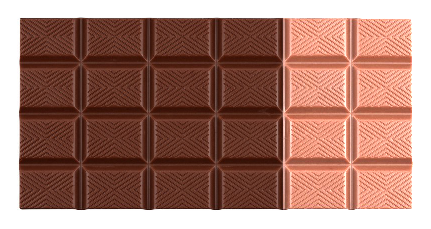
\includegraphics[width=5.25cm]{chocolat}
      \end{center}
      \begin{enumerate}
         \item Il fait un premier test sur 20 tablettes de chocolat qu'il distribue à ses amis pour la tester. \\
            Combien a-t-il besoin de chocolat en tout : trouver deux manières de calculer la masse des 20 tablettes et écrire les deux calculs {\it (aide : on peut utiliser des parenthèses dans l'un des calculs)}. \\ [3mm]
            Calcul 1 : \pf \\ [3mm]
            Calcul 2 : \pf \bigskip
         \item Ses amis trouvent qu'il n'y a pas de chocolat BR, ils proposent donc un deuxième test sur 35 tablettes de chocolat, mais en utilisant cette fois-ci \ug{56} de chocolat CI et \ug{40} de chocolat BR. \\
            Combien a-t-il besoin de chocolat en tout ? \\ [3mm]
            Calcul 1 : \pf \\ [3mm]
            Calcul 2 : \pf \bigskip
         \item Pour pouvoir effectuer ses calculs plus rapidement, il décide de trouver une formule littérale qui lui permette de calculer le nombre de carreaux de chocolat dont il aura besoin. \\
         \begin{minipage}{8cm}
            On note :
            \begin{itemize}
               \item $a$ le nombre de rangées de chocolat CI ;
               \item $b$ le nombre de rangées de chocolat BR ;
               \item $x$ le nombre de lignes de chocolat.
            \end{itemize}
         \end{minipage}
         \qquad
         \begin{minipage}{7cm}
            \psset{xunit=0.75,yunit=0.525}
            \begin{pspicture}[subgriddiv=0,gridlabels=0,gridcolor=gray](-3,-0.8)(6,4.8)
               \psgrid(0,0)(6,4)
               \psframe[linewidth=0.5mm](0,0)(6,4)
               \psline[linewidth=0.5mm](4,0)(4,4)
               \psline[linecolor=marron]{<->}(-0.3,0)(-0.3,4)
               \rput(-0.6,1.5){\textcolor{marron}{$x$}}
               \psline[linecolor=marron]{<->}(0,4.4)(4,4.4)
               \rput(2,4.8){\textcolor{marron}{$a$}}
               \psline[linecolor=marron]{<->}(4,4.4)(6,4.4)
                \rput(5,4.8){\textcolor{marron}{$b$}}
            \end{pspicture}
         \end{minipage}
         \begin{enumerate}
            \item Donner deux expressions algébriques permettant de calculer le nombre total de carreaux de chocolat. \\ [3mm]
               Calcul 1 : \pf \\ [3mm]
               Calcul 2 : \pf \bigskip
            \item Sachant que le nombre de carreaux est le même dans les deux expressions, écrire l'égalité qui résulte de ces deux calculs. \\
               \pf
         \end{enumerate}
      \end{enumerate}
   \end{QCM}
\end{activite}

%%%%%%%%%%%%%%%%%%%%%%%%%%%%%%%%%%%%%%%%%%
%%%%%%%%%%%%%%%%%%%%%%%%%%%%%%%%%%%%%%%%%%
\cours 

\section{Distributivité simple} %%%

\begin{propriete}
   Le produit d'un nombre par une somme est égal à la somme des produits de ce nombre par chacun des termes de la somme : 
   $$x \times(a+b)=x\times a+x\times b \qquad \text{ou} \qquad x(a+b) =xa+xb$$
   Le produit d'un nombre par une différence est égal à la différence des produits de ce nombre par chacun des termes de la différence : 
   $$x \times(a-b)=x\times a-x\times b \qquad \text{ou} \qquad x(a-b) =xa-xb$$
\end{propriete}

\begin{center}
   {\psset{xunit=0.9}
   \begin{pspicture}(0,-0.5)(7,2.5)
      \psframe(0,0)(5,2)
      \rput(2.5,1){$x(a+b)$}
      \psline[linecolor=B1]{<->}(-0.2,0)(-0.2,2)
      \rput(-0.5,1){\textcolor{B1}{$x$}}
      \psline[linecolor=A1]{<->}(0,2.2)(5,2.2)
      \rput(2.5,2.5){\textcolor{A1}{$a+b$}}
      \rput(6,1){\Large =}
   \end{pspicture}
   \quad
   \begin{pspicture}(0,-0.5)(5,2.5)
      \psframe(0,0)(5,2)
      \psline(4,0)(4,2)
     \rput(2,1){$xa$}
      \rput(4.5,1){$xb$}
      \psline[linecolor=B1]{<->}(-0.2,0)(-0.2,2)
      \rput(-0.5,1){\textcolor{B1}{$x$}}
      \psline[linecolor=A1]{<->}(0,2.2)(4,2.2)
      \rput(2,2.5){\textcolor{A1}{$a$}}
      \psline[linecolor=A1]{<->}(4,2.2)(5,2.2)
      \rput(4.5,2.5){\textcolor{A1}{$b$}}
   \end{pspicture}}
\end{center}

\begin{exemple}
   Calculer en ligne $8\times(12+7)$ et \\
   $17\times(100-1)$.
   \correction
      \ \\ [-10mm]
      \begin{itemize}
         \item $8\times(12+7)=8\times12+8\times7 = 96+56 =152$.
         \item $17\times(100-1)=17\times100-17\times1 =1\,700-17 =1\,683$.
      \end{itemize}
\end{exemple}


\section{Simplification d'écritures littérales} %%%

Par commutativité, on peut transformer la propriété de distributivité selon les quatre formes suivantes :
\begin{center}
   \fbox{$x(a+b) =xa+xb$} \qquad \fbox{$(a+b)x =ax+bx$} \qquad \fbox{$ax+bx=(a+b)x$} \qquad \fbox{$xa+xb =x(a+b)$} \bigskip
\end{center}

Ces différentes formes nous permettent de simplifier des écritures ou d'effectuer des calculs plus facilement.

\begin{exemple*1} 
   \mbox{} \\
   $\textcolor{B1}{13}\times102 =\textcolor{B1}{13}\times(100+2) =\textcolor{B1}{13}\times100+\textcolor{B1}{13}\times2 =1\;300+26 = 1\;326$. \\ [1mm]
   $5\,\textcolor{B1}{x}+3\,\textcolor{B1}{x} =(5+3)\,\textcolor{B1}{x} =8\,\textcolor{B1}{x}$. \\ [1mm]
   $18\,\textcolor{B1}{t}-5\,\textcolor{B1}{t}=(18-5)\,\textcolor{B1}{t}=13\,\textcolor{B1}{t}$.
\end{exemple*1}
   
\begin{center}
   \begin{pspicture}(0,0)(8,3.5)
      \psset{nodesep=2mm}
      \rput(4,1.5){\huge$ax\rnode{a}+bx = (a\rnode{b}+b)x$} 
      \nccurve[angleA=90,angleB=90,linecolor=A1]{->}{a}{b}
      \rput(3.8,3.1){\textcolor{A1}{\large factoriser}}
      \rput(8.9,1.5){\textcolor{A1}{on a mis des parenthèses}}
      \nccurve[angleA=-90,angleB=-90,linecolor=B1]{->}{b}{a}
      \rput(3.8,-0.1){\textcolor{B1}{\large développer}}
      \rput(-1.1,1.5){\textcolor{B1}{on a enlevé des parenthèses}}
   \end{pspicture}
\end{center}


%%%%%%%%%%%%%%%%%%%%%%%%%%%%%%%%%%%
%%%%%%%%%%%%%%%%%%%%%%%%%%%%%%%%%%%
\exercicesbase

\begin{colonne*exercice}

\serie{Factoriser}

\begin{exercice} %1
   Entourer le facteur commun de chaque expression, la factoriser puis calculer mentalement.
   \begin{colenumerate}{2}
      \item $83\times72+83 \times28$
      \item $36 \times25-36\times5$
      \item $98\times26+98\times4$
      \item  $16\times44-6\times44$
   \end{colenumerate}
\end{exercice}

\begin{corrige}
   \ \\ [-5mm]
   \begin{enumerate}
      \item $\fbox{83}\times72+\fbox{83} \times28 =\fbox{83}\times(72+28)$ \\
         \quad\, $=83\times100 =\blue 8\,300$ \smallskip
      \item $\fbox{36}\times25-\fbox{36}\times5 =\fbox{36}\times(25-5)$ \\
         \quad\, $=36\times20 =\blue 720$ \smallskip
      \item $\fbox{98}\times26+\fbox{98}\times4 =\fbox{98}\times(26+4)$ 
         \quad\, $=98\times30 =\blue 2\,940$ \smallskip
      \item $16\times\fbox{44}-6\times\fbox{44} =(16-6)\times\fbox{44}$ \\
         \quad\, $=10\times44 =\blue 440$
   \end{enumerate}
\end{corrige}

\bigskip
     
     
\begin{exercice} %2
   On considère l'expression suivante : \\
   $A=97\times27+3\times27$
   \begin{enumerate}
      \item En respectant les priorités opératoires, effectuer le calcul de $A$ sans  calculatrice.
      \item Factoriser $A$ puis calculer sa valeur toujours sans calculatrice.
      \item Des questions 1) et 2), quelle est la méthode la plus simple pour calculer l'expression $A$ ?
      \item Calculer sans calculatrice $B =1\,215\times47-47\times215$.
   \end{enumerate}
\end{exercice}  

\begin{corrige}
   \ \\ [-5mm]
   \begin{enumerate}
      \item $A=97\times27+3\times27 =2\,619+81 =\blue2\,700$ \smallskip
      \item $A=97\times\fbox{27}+3\times\fbox{27} =(97+3)\times\fbox{27}$ \\
         \quad\, $=100\times27 =\blue2\,700$ \smallskip
      \item La {\blue méthode 2)} est plus simple et plus rapide. \smallskip
      \item $B =1\,215\times\fbox{47}-\fbox{47}\times215$ \\
         \quad\, $=\fbox{47}\times(1\,215-215) =47\times1\,000 =\blue 47\,000$
   \end{enumerate}
\end{corrige}  

\bigskip


\begin{exercice} %3
   Factoriser chaque expression puis en donner une écriture simplifiée si nécessaire.
   \begin{colenumerate}{2}
      \item $A =6\times b+6\times d$
      \item $B =3\times4+g\times4$
      \item $C =p\times8-p\times4$
      \item $D =s\times7-4\times7$
      \item $E =6\times a+z\times 6$
      \item $F =k\times5+k\times t$ 
   \end{colenumerate}
\end{exercice}

\begin{corrige}
   \ \\ [-5mm]
   \begin{enumerate}
      \item $A =\fbox{6}\times b+\fbox{6}\times d =\blue 6(b+d)$ \smallskip
      \item $B =3\times\fbox{4}+g\times\fbox{4} =\blue 4(3+g)$ \smallskip
      \item $C =\fbox{$p$}\times8-\fbox{$p$}\times4 =\blue p(8-4) =4p$ \smallskip
      \item $D =s\times\fbox{7}-4\times\fbox{7} =\blue 7(s-4)$ \smallskip
      \item $E =\fbox{6}\times a+z\times\fbox{6} =\blue 6(a+z)$ \smallskip
      \item $F =\fbox{$k$}\times5+\fbox{$k$}\times t =\blue k(5+t)$
   \end{enumerate}
\end{corrige}

\bigskip


\begin{exercice} %4
   Faire apparaître un facteur commun puis factoriser l'expression.
   \begin{colenumerate}{2}
      \item $12+6a$
      \item $24c+12$
      \item $3x-15$
      \item $21-7g$
      \item $18b+99c$ 
      \item $7x-14y$
   \end{colenumerate}
\end{exercice}

\begin{corrige}
   \ \\ [-5mm]
   \begin{enumerate}
      \item $12+6a =\fbox{6}\times2+\fbox{6}\times a =\blue 6(2+a)$ \smallskip
      \item $24c+12 =\fbox{12}\times2c+\fbox{12}\times1 =\blue 12(2c+1)$ \smallskip
      \item $3x-15 =\fbox{3}\times x-\fbox{3}\times5 =\blue 3(x-5)$ \smallskip
      \item $21-7g =\fbox{7}\times3-\fbox{7}\times g =\blue 7(3-g)$ \smallskip
      \item $18b+99c =\fbox{9}\times2b+\fbox{9}\times11c =\blue 9(2b+11c)$ \smallskip
      \item $7x-14y =\fbox{7}\times x-\fbox{7}\times2y =\blue 7(x-2y)$ \\ [5mm]
   \end{enumerate}
\end{corrige}

\bigskip


\begin{exercice} %5
   Aurèle propose le programme de calcul suivant :
   \begin{center}
   \fbox{
   \begin{minipage}{6cm}
      \begin{itemize}
         \item Choisir un nombre.
         \item Calculer son double et son triple.
         \item Ajouter les deux nombres obtenus.
         \item Diviser le résultat par dix.
      \end{itemize}
   \end{minipage}}
   \end{center}
   \begin{enumerate}
      \item Appliquer ce programme de calcul en prenant comme nombre de départ 4 puis 15,4.
      \item Appliquer ce programme de calcul avec un nombre de votre choix.
      \item Quelle conjecture peut-on faire sur le résultat obtenu ?
      \item Montrer que la remarque reste vraie quel que soit le nombre $x$ de départ choisi.
   \end{enumerate}
\end{exercice}

\begin{corrige}
   \ \\ [-6mm]
   \begin{enumerate}
      \item \begin{pspicture}(0,-0.1)(6,0.5)
                  \rput(0.5,0){4}
                  \psline{->}(0.8,0.1)(1.8,0.4)
                  \rput{20}(1.2,0.45){\footnotesize $\times2$}
                  \rput(2.1,0.4){8}
                  \psline{->}(0.8,-0.1)(1.8,-0.4)
                  \rput{-20}(1.2,-0.4){\footnotesize $\times3$}
                  \rput(2.1,-0.4){12}
                  \psline{->}(2.4,0.4)(3.4,0.1)
                  \psline{->}(2.4,-0.4)(3.4,-0.1)
                  \rput(3,0){\footnotesize $+$}
                  \rput(3.7,0){20}
                  \psline{->}(4,0)(5,0)
                  \rput(4.4,0.25){\footnotesize $\div10$}
                  \rput(5.3,0){\blue 2}
               \end{pspicture} \\
               \quad\,
               \begin{pspicture}(0,-0.5)(6,1.5)
                  \rput(0.5,0){\small 15,4}
                  \psline{->}(0.8,0.1)(1.8,0.4)
                  \rput{20}(1.2,0.45){\footnotesize $\times2$}
                  \rput(2.1,0.4){\small 30,8}
                  \psline{->}(0.8,-0.1)(1.8,-0.4)
                  \rput{-20}(1.2,-0.4){\footnotesize $\times3$}
                  \rput(2.1,-0.4){\small 46,2}
                  \psline{->}(2.4,0.4)(3.4,0.1)
                  \psline{->}(2.4,-0.4)(3.4,-0.1)
                  \rput(3,0){\footnotesize $+$}
                  \rput(3.7,0){\small 77}
                  \psline{->}(4,0)(5,0)
                  \rput(4.4,0.25){\footnotesize $\div10$}
                  \rput(5.3,0){\blue\small 7,7}
               \end{pspicture}
   \end{enumerate}
   
   \Coupe
   
   \begin{enumerate}
      \setcounter{enumi}{1}
      \item \begin{pspicture}(0,-0.1)(6,0.9)
                  \rput(0.5,0){0}
                  \psline{->}(0.8,0.1)(1.8,0.4)
                  \rput{20}(1.2,0.45){\footnotesize $\times2$}
                  \rput(2.1,0.4){0}
                  \psline{->}(0.8,-0.1)(1.8,-0.4)
                  \rput{-20}(1.2,-0.4){\footnotesize $\times3$}
                  \rput(2.1,-0.4){0}
                  \psline{->}(2.4,0.4)(3.4,0.1)
                  \psline{->}(2.4,-0.4)(3.4,-0.1)
                  \rput(3,0){\footnotesize $+$}
                  \rput(3.7,0){0}
                  \psline{->}(4,0)(5,0)
                  \rput(4.4,0.25){\footnotesize $\div10$}
                  \rput(5.3,0){\blue 0}
               \end{pspicture} \\
      \item On obtient à chaque fois {\blue la moitié du nombre}.
      \item \begin{pspicture}(0,-0.1)(6,0.9)
                  \rput(0.5,0){$x$}
                  \psline{->}(0.8,0.1)(1.8,0.4)
                  \rput{20}(1.2,0.45){\footnotesize $\times2$}
                  \rput(2.1,0.4){$2x$}
                  \psline{->}(0.8,-0.1)(1.8,-0.4)
                  \rput{-20}(1.2,-0.4){\footnotesize $\times3$}
                  \rput(2.1,-0.4){$3x$}
                  \psline{->}(2.4,0.4)(3.4,0.1)
                  \psline{->}(2.4,-0.4)(3.4,-0.1)
                  \rput(3,0){\footnotesize $+$}
                  \rput(3.7,0){$5x$}
                  \psline{->}(4,0)(5,0)
                  \rput(4.4,0.25){\footnotesize $\div10$}
                  \rput(5.5,0){\blue $0,5x$}
               \end{pspicture} \\
   \end{enumerate}
\end{corrige}

\bigskip


\serie{Développer} %%%%%%%%%%

\begin{exercice} %6
   \begin{enumerate}
      \item Sans calculatrice, poser le calcul suivant : \\
      $E =33\times103$.
      \item Décomposer le nombre 103 comme une somme de deux nombres simples. 
      \item Développer l'expression $E$ et effectuer les calculs.
      \item Quelle est la méthode la plus simple pour calculer l'expression $E$ de tête ?
   \end{enumerate}
\end{exercice}

\begin{corrige}
   \ \\ [-7mm]
   \begin{enumerate}
      \item On peut poser la multiplication : \qquad $\opmul[voperation=top,voperator=top]{103}{33}$ \\
         On trouve $33\times103 =103\times33 =\blue 3\,399$
      \item $103 =\blue 100+3$
      \item $E =33\times(100+3) =33\times100+33\times3$ \\
         \quad\, $=3\,300+99 =\blue 3\,399$
      \item La {\blue méthode par décomposition} est plus simple pour calculer le résultat de tête.
   \end{enumerate}
\end{corrige}

\bigskip


\begin{exercice} %7
   On donne : $197\times17 =3\,349$ et $197\times4 =788$. \\
   Calculer les nombres suivants en proposant une décomposition qui utilise les égalités ci-dessus.
   \begin{colenumerate}{2}
      \item $A =197\times21$
      \item $B =197\times13$
      \item $C =197\times34$
      \item $D =197\times12$
   \end{colenumerate}
\end{exercice}

\begin{corrige}
   \ \\ [-5mm]\begin{enumerate}
      \item $A =197\times21 =197\times(17+4) $\\
         \quad\, $=197\times17+197\times4 =3\,349+788 =\blue 4\,137$
      \item $B =197\times13 =197\times(17-4)$ \\
         \quad\, $=197\times17-197\times4 =3\,349-788 =\blue 2\,561$
      \item $C =197\times34 =197\times(17\times2)$ \\
         \quad\, $=(197\times17)\times2 =3\,349\times2 =\blue 10\,047$
      \item $E =197\times12 =197\times(4\times3)$ \\
         \quad\, $=(197\times4)\times3 =788\times3 =\blue 6\,698$
   \end{enumerate}
\end{corrige}

\bigskip


\begin{exercice} %8
   Développer chaque expression puis en donner une écriture simplifiée.
   \begin{colenumerate}{2}
      \item $A =5\times(a+9)$
      \item $B =3\times(10+b)$
      \item $C =(11+c)\times7$
      \item $D =2\times(a-4)$
      \item $E =(9,3-c)\times5$
      \item $F =4\times(a+b)$
   \end{colenumerate}
\end{exercice}

\begin{corrige}
   \ \\ [-5mm]
   \begin{enumerate}
      \item $A =5\times(a+9) =5\times a+5\times9 =\blue 5a+45$
      \item $B =3\times(10+b) =3\times10+3\times b =\blue 30+3b$
      \item $C =(11+c)\times7 =11\times7+c\times7 =\blue 77+7c$
      \item $D =2\times(a-4) =2\times a-2\times4 =\blue 2a-8$
      \item $E =(9,3-c)\times5 =9,3\times5-c\times5 =\blue 46,5-5c$
      \item $F =4\times(a+b) =4\times a+4\times b =\blue 4a+4b$
   \end{enumerate}
\end{corrige}

\bigskip


\begin{exercice} %9
   Millie propose le programme de calcul suivant :
   \begin{center}
   \fbox{
   \begin{minipage}{6cm}
      \begin{itemize}
         \item Choisir un nombre.
         \item Calculer son triple.
         \item Ajouter 5
         \item Doubler le résultat obtenu.
      \end{itemize}
   \end{minipage}}
   \end{center}
   \begin{enumerate}
      \item Appliquer ce programme de calcul en prenant comme nombre de départ 4 puis 1,5.
      \item Effectuer ce programme pour un nombre $x$ de départ et écrire une expression simplifiée du résultat en fonction de $x$.
      \item Utiliser cette expression pour calculer le résultat \\ [1mm] obtenu à partir du nombre $\dfrac72$ puis du nombre $0$. \\ [5mm]
   \end{enumerate}
\end{exercice}

\begin{corrige}
   \ \\ [-5mm]
   \begin{enumerate}
      \item $4\;\stackrel{\times3}{\longrightarrow}\;12\;\stackrel{+5}{\longrightarrow}\;17\;\stackrel{\times2}{\longrightarrow}\;\blue 34$ \\ \medskip
         \quad\, $1,5\;\stackrel{\times3}{\longrightarrow}\;4,5\;\stackrel{+5}{\longrightarrow}\;9,5\;\stackrel{\times2}{\longrightarrow}\blue 19$ \\ \medskip
      \item $x\;\stackrel{\times3}{\longrightarrow}\;3x\;\stackrel{+5}{\longrightarrow}\;3x+5\;\stackrel{\times2}{\longrightarrow}\;2(3x+5) =\blue 6x+10$ \\ \medskip
      \item $6\times\dfrac72+10 =\dfrac{42}{2}+10 =21+10 =\blue 31$ \\ \medskip
      \quad\, $6\times0+10 =0+10 =\blue 10$ \\
   \end{enumerate}

\Coupe
\bigskip

\corec{Un diamant algébrique}

{\psset{unit=2.5}
      \begin{pspicture}(-0.107,0)(6,8)      
         \rput{-60}(2,4){\tri{7(x+10)}{14x-35}{14x+140}}
         \rput(2,4){\tri{7(2x-5)}{14x+35}{7(x+5)}}
         \rput{60}(2,4){\car{7(2x+5)}{2x-4}{}{4(x-2)}}
         \rput{150}(2,4){\tri{4x-8}{5(4x+1)}{}}
         \rput{-150}(2,4){\car{20x+5}{}{10(2x+1)}{7x+70}}
         \rput{-150}(3,2.27){\tri{20x+10}{10(x+2)}{}}
         \rput{-90}(3,2.27){\tri{10x+20}{10(x+1)}{}}
         \rput{-120}(4,4){\car{14(x+10)}{10x+10}{}{5(2x+1)}}
         \rput{-30}(4,4){\tri{10x+5}{4(4x-1)}{}}
         \rput{30}(4,4){\car{16x-4}{}{4(2x-1)}{7x+35}}
         \rput{30}(3,5.73){\tri{8x-4}{2(x-1)}{}}
         \rput{90}(3,5.73){\tri{2x-2}{2(x-2)}{}}
      \end{pspicture}}   
\end{corrige}

\hfill {\it\footnotesize Source : d’après Les cahiers Sésamath 5e. Magnard-Sésamath 2017.}

\end{colonne*exercice}


%%%%%%%%%%%%%%%%%%%%%%%%%%%%%%%%%%%%%%%%%%
\Recreation

\newcommand{\tri}[3]{\pspolygon(0,0)(2,0)(2;60) \rput(1,0.25){$#1$} \rput{-120}(0.7,0.8){$#2$} \rput{120}(1.3,0.8){$#3$}}
\newcommand{\car}[4]{\psframe(0,0)(2,2) \rput(1,0.2){$#1$} \rput{90}(1.8,1){$#2$} \rput{180}(1,1.8){$#3$} \rput{-90}(0.2,1){$#4$}}

\enigme[Un diamant algébrique]
   \begin{minipage}{9cm}
      Découper les douze pièces du puzzle et les assembler de telle sorte que les expressions face à face soient égales. Coller le puzzle sur votre cahier. \\ [2mm]
      La forme à obtenir est celle ci-contre.
   \end{minipage}
   \hfill
   \begin{minipage}{5cm}
      {\psset{unit=0.5}
      \begin{pspicture}(0,1)(6,7)      
         \rput{-60}(2,4){\tri{}{}{}}
         \rput(2,4){\tri{}{}{}}
         \rput{60}(2,4){\car{}{}{}{}}
         \rput{150}(2,4){\tri{}{}{}}
         \rput{-150}(2,4){\car{}{}{}{}}
         \rput{-150}(3,2.27){\tri{}{}{}}
         \rput{-90}(3,2.27){\tri{}{}{}}
         \rput{-120}(4,4){\car{}{}{}{}}
         \rput{-30}(4,4){\tri{}{}{}}
         \rput{30}(4,4){\car{}{}{}{}}
         \rput{30}(3,5.73){\tri{}{}{}}
         \rput{90}(3,5.73){\tri{}{}{}}
      \end{pspicture}}
   \end{minipage}
   \begin{center}
      {\psset{unit=2.5,linewidth=0.6mm}
      \large
      \begin{pspicture}(0,-0.5)(6,6.5)
         \rput(0,0){\car{4(x-2)}{7(2x+5)}{2x-4}{}}
         \rput(2,0){\car{7x+35}{16x-4}{}{4(2x-1)}}
         \rput(4,0){\car{20x+5}{}{10(2x+1)}{7x+70}}
         \rput(0,2){\tri{}{4x-8}{5(4x+1)}}
         \rput{60}(2,2){\tri{14x+140}{7(x+10)}{14x-35}}
         \rput(2,2){\tri{}{10x+5}{4(4x-1)}}
         \rput{60}(4,2){\tri{7(x+5)}{7(2x-5)}{14x+35}}
         \rput(4,2){\tri{}{2x-2}{2(x-2)}}
         \rput(0,3.73){\car{14(x+10)}{10x+10}{}{5(2x+1)}}
         \rput(2,3.73){\tri{8x-4}{2(x-1)}{}}
         \rput{60}(4,3.73){\tri{10x+20}{10(x+1)}{}}
         \rput(4,3.73){\tri{}{20x+10}{10(x+2)}}
      \end{pspicture}}
   \end{center}
   \vfill \hfill{\it\footnotesize Source : \href{https://www.monclasseurdemaths.fr/profs/puzzles/}{monclasseurdemaths.fr}}
